\documentclass[../main/main.tex]{subfiles}
\begin{document}

\chapter{Geometry in the spacetime}
Refer to \textsf{Carroll chap. 2} and \textsf{Nakahara chap. 5,7} for this chapter.\\

\section{Manifolds}

\begin{definition}[Manifold]{}
$M$ is a $d$-dimensional differentiable manifold if
\begin{enumerate}
\item $M$ is a topological space
\item $M$ is provided with a family of pairs $\{(U_\alpha, \phi_\alpha)\}$
\item $\{U_\alpha\}$ is a family of open sets which covers $M$, that is,  $\bigcup_\alpha U_\alpha=M$. $\phi_\alpha$ is a homeomorphism from $U_\alpha$ onto an open subset $U_\alpha'$ of $\RR^d$;  
\begin{figure}[H]
\centering
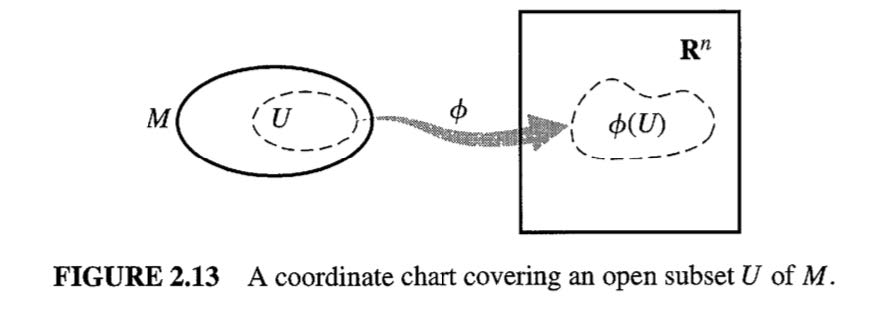
\includegraphics[width=7cm]{../img/chart-diff-geo.jpg}
\end{figure}
\item given $U_\alpha$ and $U_\beta$ such that $U_\alpha\cap U_\beta\neq\emptyset$, the map $\psi_{\alpha\beta}=\phi_\alpha\circ\phi_\beta^{-1}$ from $\phi_\beta(U_\alpha\cap U_\beta)$ to $\phi_\alpha(U_\alpha\cap U_\beta)$ is infinitely differentiable.
\begin{figure}[H]
\centering
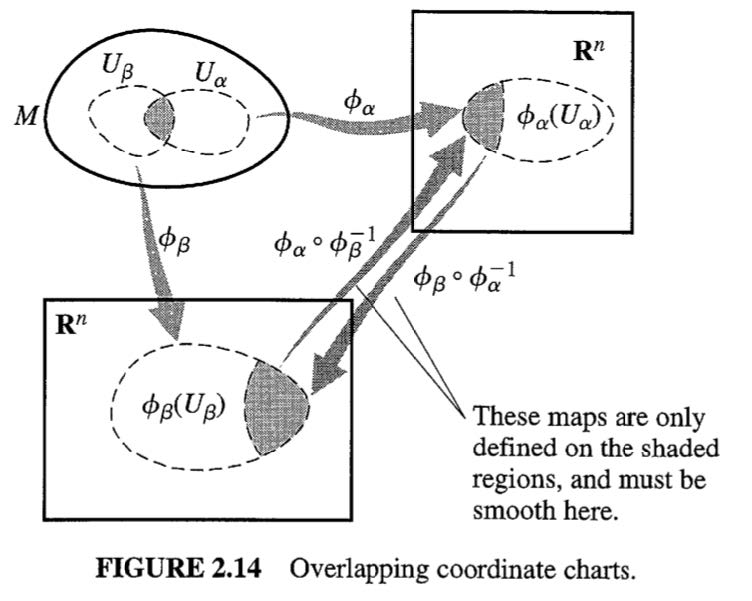
\includegraphics[width=7cm]{../img/compatible-chart-diff-geo.jpg}
\end{figure}
\end{enumerate}
The pair $(U_\alpha, \phi_\alpha)$ is called a \textbf{chart} while the whole family $\{(U_\alpha, \phi_\alpha)\}$ is called an \textbf{atlas}. The subset $U_\alpha$ is called the \textbf{coordinate neighbourhood} while $\phi_\alpha$ is the \textbf{coordinate function} or, simply, the \textbf{coordinate}. If $U_\alpha$ and $U_\beta$ overlap, two coordinate systems are assigned to a point in $U_\alpha\cap U_\beta$. Axiom (iv) asserts that the transition from one coordinate system to another be \emph{smooth} ($C^\infty$). The map $\psi_{\alpha\beta}=\phi_\alpha\circ\phi_\beta^{-1}$ is called \textbf{transition function}. The choice of an atlas is not unique, in particular for each manifold there are infinite equivalent choices of atlas. If the union of two atlases $\{(U_\alpha, \phi_\alpha)\}$ and $\{(V_\beta, \varphi_\beta)\}$ is again an atlas, these two atlases are said to be \textbf{compatible}. The compatibility is an equivalence relation, the equivalence class of which is called the \textbf{differentiable structure}.
\end{definition}

\begin{example}[$S^2$]
The two dimensional sphere $S^2$ given by the subset of $\RR^3$ defined by the equation
\[(X^1)^2+(X^2)^2+(X^3)^2=R^2\]
is a differentiable manifold. Notice that no single chart is possible, since the sphere is a closed set, thus cannot be found any homeomorphism with an open set of $\RR^2$, rather we need to define at least two charts. We can do this using \emph{stereographic coordinates}:
\begin{alignat*}{4}
\phi_N\,:\,U_N=&&S^2\setminus\{(0,0,-R)\}&&\quad\longrightarrow\quad &\phi_N(U_N)\simeq\RR^2\\
&&(X^1,X^2,X^3)&&\quad\longmapsto\quad&\p{x_N^1=\frac{2X^1}{R+X^3},\,x_N^2=\frac{2X^2}{R+X^3}}
\end{alignat*}
\begin{figure}[H]
\centering
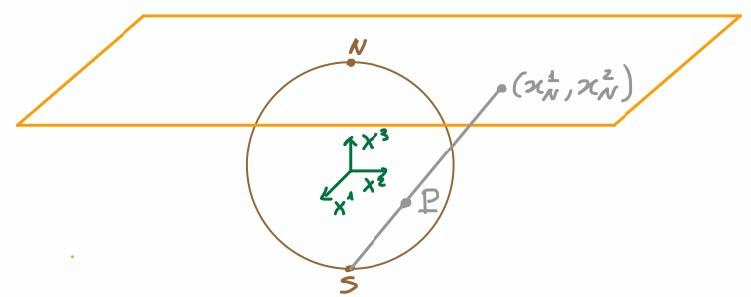
\includegraphics[width=7cm]{../img/stereo-coord-2sphere.jpg}
\end{figure}
\noindent where the chart is defined for all points of $S^2$ beside the south pole. Analogously, removing the north pole:
\begin{alignat*}{4}
\phi_S\,:\,U_S=&&S^2\setminus\{(0,0,R)\}&&\quad\longrightarrow\quad &\phi_S(U_S)\simeq\RR^2\\
&&(X^1,X^2,X^3)&&\quad\longmapsto\quad&\p{x_S^1=\frac{2X^1}{R-X^3},\,x_S^2=\frac{2X^2}{R-X^3}}
\end{alignat*}
We can see that transition functions are smooth:
\begin{align*}
\phi_S\circ\phi_N^{-1}\,:\,(x_N^1,x_N^2)\quad\longmapsto\quad	 \begin{cases}
x_S^1=\frac{4x_N^1}{(x_N^1)^2+(x_N^2)^2}\\
x_S^2=\frac{4x_N^1}{(x_N^2)^2+(x_N^2)^2}
\end{cases}
\end{align*}
\end{example}

\begin{example}[$S^n$]
The two dimensional sphere $S^n$ given by the subset of $\RR^{n+1}$ defined by the equation
\[(X^1)^2+(X^2)^2+\dots+(X^{n+1})^2=R^2\]
is a differentiable manifold. Notice that again no single chart is possible, rather we need to define several charts. This time, instead of stereographic coordinates (which works too) we use \emph{angular coordinates}:
\begin{align*}
\begin{cases}
X^{n+1}&=R\cos\theta_1\\
X^n&=R\sin\theta_1\cos\theta_2\\
X^{n-1}&=R\sin\theta_1\sin\theta_2\cos\theta_3\\
&\vdots\\
X^2&=R\sin\theta_1\dots\cos\theta_n\\
X^1&=R\sin\theta_1\dots\sin\theta_n
\end{cases}
\qquad\text{with}\quad0<\theta_1,\dots,\theta_{n-1}<\pi\,,\quad0<\theta_n<2\pi
\end{align*}
\begin{figure}[H]
\centering
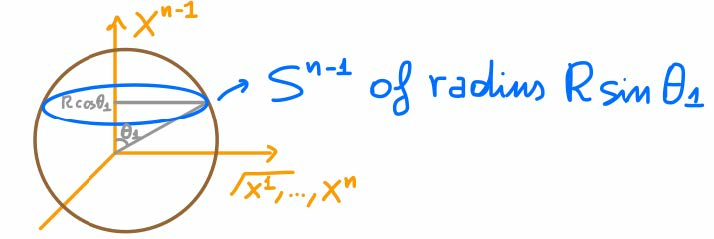
\includegraphics[width=8cm]{../img/chart-N-sphere-angular.jpg}
\end{figure}
\noindent Notice that this coordinates degenerate at $\theta_1,\dots,\theta_{n-1}=0,\pi$, therefore this chart do not cover the entire $S^n$. For example coordinates for the submanifold $S^{n-2}=S^n\cap\{X^1=X^2=0\}$ (i.e. $\theta_{n-1}=0$) are not well defined. In order to cover the full sphere we can use charts with ``rotated'' angular coordinates that covers subsets of $S^n$ where the previous chart is not well defined. 

\end{example}


\begin{example}[$n$-dim. de Sitter spacetime]
The so called \textbf{$n$-dim. de Sitter spacetime}, indicated by dS$n$, is the manifold defined as the subset of  $R^{n+1}$ with equation:
\[|\vec X|^2-T^2=L^2\]
where $\vec X=(X^1,\dots,X^n)$ are $n$ space coordinates while $T$ is a time coordinate. 
\begin{figure}[H]
\centering
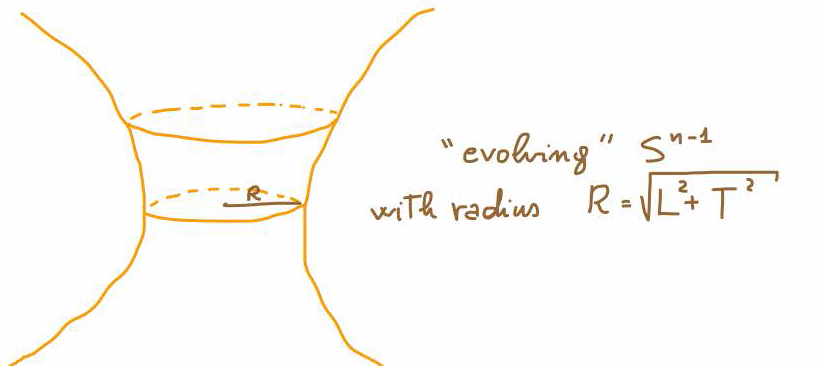
\includegraphics[width=8cm]{../img/de-Sitter-manifold.jpg}
\end{figure}
\noindent It's clear that this manifold takes the form of an hyperboloid. 
We may also introduce local coordinates on the manifold $x^\mu=(x^0,x^i)=(t,x^i)$. First we introduce coordinates $t$ and $\hat X^I$ such that
\begin{align*}
T&=L\sinh t\\
X^I&=L\cosh \hat X^I
\end{align*}
with $\sum_{I=1}^n(\hat X^I)^2=1$, i.e. coordinates $\{\hat X^I\}$ define a sphere $\hat S^{n-1}$ with radius $\hat R=1$. Then, $\hat S^{n-1}$ can be covered using some atlas (e.g. using stereographic or angular coordinates), defining local coordinates $\{x^i\}$ on $\hat S^{n-1}$. In this way, taking into account also $x^0=t$, we introduce coordinates $x^\mu$ over dS$n$. \\
What we have done is just slice dS$n$ into spheres (circumferences in the figure) and then parametrize them as we already know by previous examples. 

\end{example}

Up to this point, we want to stress the fact that for these manifolds only pathches, topological and differential structure have been specified. No notion of distance has been introduced yet. 


\section{Calculus on Manifolds}


\begin{definition}[Scalar field]{}
A \textbf{scalar field} is defined as a function
\begin{alignat*}{4}
F\,:\,&&M&&\quad\longrightarrow\quad&\RR\qquad(\text{or }\CC)\\
&&p&&\quad\longmapsto\quad&F(p)
\end{alignat*}
Let $(U,\phi)$ be a patch for $M$ with local coordinates $x^\mu$, then for each $p\in U$ we can define the \emph{local form} of F
\begin{alignat*}{4}
f=F\circ\phi^{-1}\,:\,&&\RR^d&&\quad\longrightarrow\quad&\RR\qquad(\text{or }\CC)\\
&&x&&\quad\longmapsto\quad&F(\phi^{-1}(x))
\end{alignat*}
If we consider a different patch $(\tilde U,\tilde \phi)$ associated to local coordinates $\tilde x^\mu$, and the local form of $f$ in this patch $\tilde f=F\circ\tilde\phi^{-1}$, then its immediate that following \textbf{transformation rule for a scalar field} holds:
\[\boxed{\tilde f(\tilde x)=f(x)}\]
where $\tilde x$ are the coordinates for $M$ using the patch $(\tilde U,\tilde \phi)$.
\end{definition}

Pragmatically, we will not distinguish between $F(p)$ and its local form $f(x)$ and use the latter.
%
\begin{definition}[Vector field]{}
We define a \textbf{vector field}
\begin{alignat*}{4}
V\,:\,&&M&&\quad\longrightarrow\quad&TM\\
&&p&&\quad\longmapsto\quad& V^\mu(p)\partial_\mu\big\vert_p
\end{alignat*}
where $V^\mu$ is a set of  functions called \textbf{components of the vector field} and $\partial_\mu\equiv\frac\partial{\partial x^\mu}\vert_p$ are partial derivatives defined respect to the local coordinates in $p$ given by some patch, and they can be applied to any scalar field. The set $TM$ is a set of derivative operators that will be defined later. If functions $V^\mu$ are differentiable then the vector field is said \textbf{smooth}, and this condition is independent from the choice of the patch. The element $V(p)$ for some point $p\in M$ is said to be a  \textbf{vector in $p$} and the set of all vectors attached to a point $p$ (for all possible vector fields) is called \textbf{tangent space in $p$}, denoted by $T_pM$. Each $V^\mu(p)\partial_\mu\vert_p$ can be interpreted as a vector in $p$ with components $(V^1(p),V^2(p),\dots,V^n(p))$.

Suppose that $x^\mu$ and $\tilde x^\mu$ are local coordinates on two subsets $U$ and $\tilde U$. 
Notice that since transition functions for different charts are smooth, then in $U\cap\tilde U$ the Jacobian of the transition function $\frac{\partial\tilde x^\mu}{\partial x^\nu}(p)$ must be invertible, with inverse $\frac{\partial x^\mu}{\partial\tilde x^\nu}(p)$. The transformation rule for partial derivatives is then given by the differentiable application $\partial_\mu=\frac{\partial\tilde x^\nu}{\partial x^\mu}\tilde\partial_\nu$ and similarly the \textbf{transformation rule for a vector field} is 
\[\hspace{1cm}
\begin{split}
 &V^\mu\partial_\mu=V^\mu\frac{\partial\tilde x^\nu}{\partial x^\mu}\tilde\partial_\nu=\tilde V^\nu\tilde\partial_\mu\\
&\boxed{\tilde V^\mu(\tilde x)=\frac{\partial\tilde x^\mu}{\partial x^\nu}V^\nu(x)}
\end{split}
\hspace{1cm}
\raisebox{-2cm}{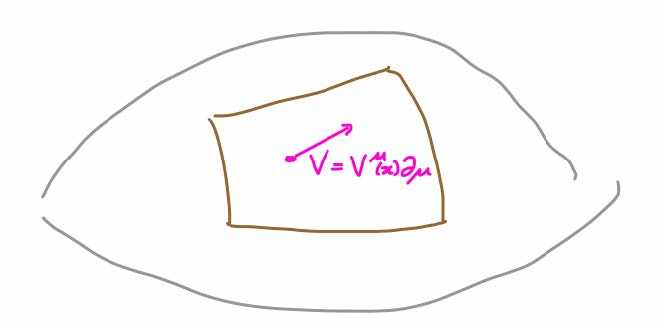
\includegraphics[width=5.5cm]{../img/tangent-vector.jpg}}
\]
Notice that this application reduce to the Minkowski rule for Poincaré transformations $\tilde x^\mu={\Lambda^\mu}_\nu x^\nu+\alpha^\mu$. 
Here is a pictorial representation of a smooth vector field on a sphere:
\begin{figure}[H]
\centering
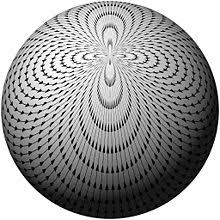
\includegraphics[width=5cm]{../img/example-vector-field.jpg}
\end{figure}

Starting from a manifold $M$ and a vector field $V$, we can define \textbf{integral curves}
\begin{alignat*}{4}
\gamma\,:\,&&\RR\supset I&&\quad\longrightarrow\quad&\gamma(I)\subset M\\
&&\lambda&&\quad\longmapsto\quad &\gamma(\lambda)
\end{alignat*}
such that
\[\frac{\de \gamma^\mu}{\de\lambda}(\lambda)=V^\mu(\gamma(\lambda))\]
\begin{figure}[H]
\centering
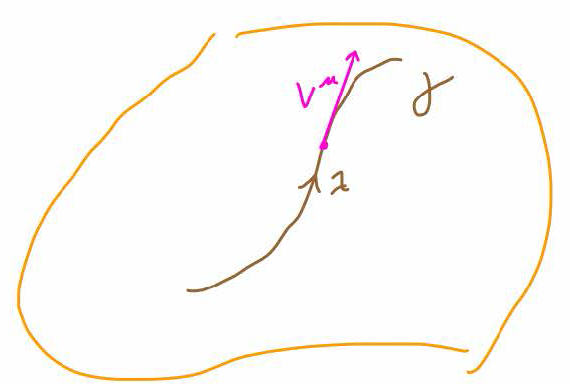
\includegraphics[width=4cm]{../img/integral-curve.jpg}
\end{figure}
\noindent Notice that the latter equation describes a set of first order differential equations with unique solution for a given initial conditions. The set of all integral curves, for different initial coordinates, is called the \textbf{flow} of the vector field.
\begin{figure}[H]
\centering
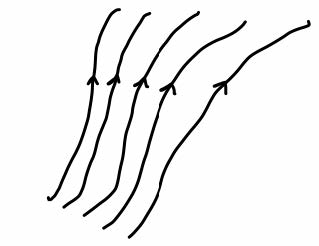
\includegraphics[width=2.5cm]{../img/flow-vector-field.jpg}
\end{figure}
\noindent We can then regard $V(p)$ as defining a directional derivative in $p$ of any smooth scalar field $f$ along the integral curve of $V$ that goes through $p=\gamma(\lambda_p)$ :
\[V(f)(p)\equiv V^\mu(p)\partial_\mu f(p)=\frac{\de \gamma^\mu}{\de\lambda}(p)\partial_\mu f(p)=\frac{\de (f\circ\gamma)}{\de\lambda}(\lambda_p)\]
and this can be interpreted as the derivative of the restriction of $f$ along $\gamma$. This also allows a better interpretation of tangent vectors as derivative operators that can be applied to scalar fields. 

At each point $p\in M$ the tangent space $T_pM$ is a $d$-dimensional vector space and $\partial_\mu\big\vert_p\equiv\frac\partial{\partial x^\mu}\big\vert_p$ provide the coordinate basis associated with the local coordinates $x^\mu$, called \textbf{coordinate basis}. However we could take any other basis of linearly independent vectors $e_a=e_a^\mu(x)\partial_\mu\in T_pM$, $a=1,\dots,d$ so that $V(x)=V^a(x)e_a=V^\mu(x)\partial_\mu$ with $V^\mu(x)=e_a^\mu(x)V^a(x)$. Often indices $a$ are called \emph{``local''} (or \emph{``flat''} in GR) \emph{indices}, while $\mu$ are called \emph{``curved'' indices}.

The collection of the tangent spaces in each point $p\in M$ is called \textbf{tangent bundle} $TM$
\[TM=\bigcup_{p\in M}T_pM
\hspace{1.5cm}
\raisebox{-1cm}{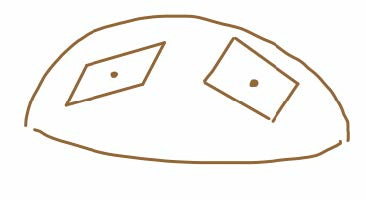
\includegraphics[width=3cm]{../img/vector-bundle.jpg}}
\]
\noindent Notice that this is a $2d$-dimensional manifold. A vector field $V$ can be also define as a function between the manifold and a bundle, i.e. a \textbf{section}. In particular a vector field is a section of the vector bundle
\begin{alignat*}{4}
V\,:\,&&M&&\quad\longrightarrow\quad&TM\\
&&p&&\quad\longmapsto\quad &X_p\in T_pM
\end{alignat*}
\end{definition}

\begin{example}
Let's consider the vector field $V=\sin\theta\partial_\phi$ where we used spherical coordinates $(x^1,x^2)=(\theta,\phi)$. Its components are
\vspace{-0.5cm}
\[V^\mu=(V^1,V^2)\equiv(V^\theta, V^\phi)=(0,\sin\theta)
\hspace{0.5cm}
\raisebox{-2cm}{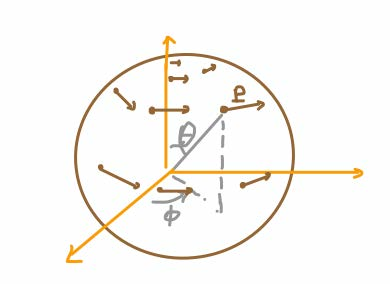
\includegraphics[width=4cm]{../img/vector-field-sintheta.jpg}}
\]
\end{example}

\begin{definition}[One-forms]{}

One can consider another kind of vector fields $\alpha_\mu$, called \textbf{1-forms}, which transforms in the ``dual'' way, i.e. follows following \textbf{transformation rule of one-forms}:
\[\boxed{
\tilde\alpha_\mu(\tilde x)=\frac{\partial x^\nu}{\partial\tilde x^\mu}\alpha_\nu(x)
}\]
Notice that since this transformation is the inverse of the one we defined for vector fields, then the product between a 1-form and a vector space is invariant under transformations, i.e. is a scalar
\[\alpha_\mu(x)V^\mu(x)=(x)\]
This proprieties suggests a  more intrinsic definition of a one-form field, which assigns at any $p\in M$ an element $\alpha$ of the \textbf{cotangent space}
\begin{align*}
T^*_pM&=\{\text{vector space \textbf{dual} to }T_pM\}\\
=\{\text{space of linear functionals $\alpha$ on }T_pM\}
\end{align*}
hence
\[\alpha\,:\, V\in  T_pM\quad\longmapsto \quad\alpha(V)\in\RR\]
such that
\[\alpha(aV_1+bV_2)=a\alpha(V_1)+b\alpha(V_2)\]
The coordinate basis dual to basis $\partial_\mu\in T_pM$ is given by
\[\de x^\mu\in T^*_p M\quad \forall p\in U\quad\text{such that} \quad\de x^\mu(\partial_\nu)=\delta^\mu_\nu\]
Respect to this basis a generic one-form we can write as $\alpha=\alpha_\mu(x)\de x^\mu$, so is action is described by
\[\alpha(V)=\alpha(V^\mu(x)\partial_\mu)=V^\mu(x)\alpha_\nu(x)\de x^\nu(\partial_\mu)=\alpha_\mu(x)V^\mu(x)\]
The last description in terms of the basis leads to an interpretation of one forms as linear combinations of infinitesimal coordinate variations. Indeed the transformation rule for one-forms is the same as the transformation rules for line elements
\[\de \tilde x^\mu=\frac{\partial \tilde x^\mu}{\partial x^\nu}\de x^\nu\quad\Rightarrow
\quad\tilde \alpha(\tilde x)=\tilde\alpha_\mu(\tilde x)\de\tilde x^\mu=\alpha_\mu(x)\de x^\mu=\alpha(x)\]

One can also take arbitrary basis of linearly independent 1-forms:
\[\boxed{
e^a=e^a_\mu(x)\de x^\mu\in T^*_pM	\qquad a=1,\dots,\quad\forall p\in M
}\]
In order to be consistent with the representation in terms of coordinate basis we must have
\[\alpha(x)=\alpha_a(x)e^a=\alpha_\mu(x)\de x^\mu\]
therefore
\[\alpha_\mu(x)=e^a_\mu(x)\alpha_a(x)\]

A particular subclass of one forms is given by \textbf{exact 1-forms}
\[\alpha(x)\de f(x)=\partial_\mu f(x)\de x^\mu\qquad f(x)\text{ scalar field}\]
that in components implies $\alpha_\mu(x)=\partial_\mu f(x)$.

Observe that 
\[\de f(V)=\partial_\mu f V^\mu\]
gives the \textbf{directional derivative} of $f$ along $V$.

A one-form field $\alpha$ assigns an element of $T^*_p$ at each $p\in M$. This can be considered as a section of the \textbf{cotangent bundle}
\[T^*M\equiv\bigcup_pT^*_pM\]

\end{definition}


\begin{definition}[General tensors]{}

Pragmatically, a \textbf{tensor field of type ($n,m$)} is a field characterized $n$ upper indices and $n$ lower indices
\[{T^{\mu_1\dots\mu_n}}_{\nu_1\dots\nu_m}(x)\]
In order to define such a field over an entire manifold one can define how this fields transforms under coordinate transformation, namely the \textbf{transformation rule for tensor fields}:
\[\boxed{
{\widetilde T^{\mu_1\dots\mu_n}\,}_{\nu_1\dots\nu_m}(\tilde x)=
\frac{\partial \tilde x^{\mu_1}}{\partial x^{\rho_1}}\dots\frac{\partial \tilde x^{\mu_n}}{\partial x^{\rho_n}}\frac{\partial  x^{\sigma_1}}{\partial \tilde x^{\nu_1}}\dots\frac{\partial  x^{\sigma_m}}{\partial \tilde x^{\nu_m}}{T^{\rho_1\dots\rho_n}}_{\sigma_1\dots\sigma_m}(x)
}\]
More intrinsically, a tensor fields at each point $p\in M$ is an element of the vector space
\[(T_pM)^{\otimes n}\otimes(T_p^*M)^{\otimes m}\]
Then we can express the tensor fields in terms of coordinate basis or an arbitrary local basis either:
\begin{align*}
T(x)&={T^{\mu_1\dots\mu_n}}_{\nu_1\dots\nu_m}(x)\,\partial_{\mu_1}\otimes\dots\otimes\partial_{\mu_n}\otimes\de x^{\nu_1}\otimes\dots\otimes\de x^{\nu_m}\\
&={T^{a_1\dots a_n}}_{b_1\dots b_m}(x)\,e_{a_1}\otimes\dots\otimes e_{a_n}\otimes e^{b_1}\otimes\dots\otimes e^{b_m}
\end{align*}
where this time ${T^{\mu_1\dots\mu_n}}_{\nu_1\dots\nu_m}(x)$ and ${T^{a_1\dots a_n}}_{b_1\dots b_m}(x)$ are a set of functions and are required to satisfy the equality between two transformations.

Some tensors  may have specific index-symmetries, for instance 
\[{S^\mu}_{\nu\rho}={S^\mu}_{\rho\nu}\]
is \textbf{symmetric} in second and third indices, while
\[A^{\mu\nu\rho}=-A^{\mu\rho\nu}\]
is \textbf{antisymmetric} in second and third indices. Notice that tensors with $>d$ antisymmetric indices is identically vanishing.

Given a tensor, one can \textbf{symmetrize} or \textbf{antisymmetrize} any number of upper or lower indices
\begin{align*}
{{T_\rho}^\sigma}_{\mu_1\dots\mu_n}\quad&\longrightarrow\quad {{T_\rho}^\sigma}_{(\mu_1\dots\mu_n)}=
\frac1{n!}({{T_\rho}^\sigma}_{\mu_1\dots\mu_n}\,+\text{ permutations of }\mu_1\dots\mu_n)\\
{{T_\rho}^\sigma}_{\mu_1\dots\mu_n}\quad&\longrightarrow\quad {{T_\rho}^\sigma}_{[\mu_1\dots\mu_n]}=
\frac1{n!}({{T_\rho}^\sigma}_{\mu_1\dots\mu_n}\,\pm\text{ permutations of }\mu_1\dots\mu_n)
\end{align*}
where in the second case we take positive sign when we sum an element obtained by an even permutation of indices, while we take munis sign when we sum an element obtained by ad odd permutation of indices.
For instance
\begin{align*}
T_{(\mu\nu)}&=\frac12(T_{\mu\nu}+T_{\nu\mu})\\
T_{[\mu\nu]}&=\frac12(T_{\mu\nu}-T_{\nu\mu})
\end{align*}
The factor $\frac1{n!}$ is inserted in such a way that if the initial tensor is already (anti)symmetric then its (anti)symmetrized tensor is the same as the initial one. 

\end{definition}


\begin{definition}[Differential forms]{}

A distinguish subclass of tensor fields is given by the ``{forms}''
\[A_{\mu_1\dots\mu_p}(x)=A_{[\mu_1\dots\mu_p]}(x)\]
i.e. total antisimmetric tensors, called \textbf{$p$-forms} where $p$ is the degree of the form (recall that $p\leq d$, otherwise the form vanishes).

For this class of tensor is useful to introduce a special basis obtained by taking \textbf{wedge-product} of the one form basis
\begin{align*}
\de x^{\mu_1}\wedge\de x^{\mu_2}\wedge\dots\wedge\de x^{\mu_p}
&=p!\,\de x^{[\mu_1}\otimes\de x^{\mu_2}\otimes\dots\otimes\de x^{\mu_p]}\\
&=(\de x^{\mu_1}\otimes\de x^{\mu_2}\otimes\dots\otimes\de x^{\mu_p}\,+\text{ permutations with alternating signs })
\end{align*}
where $p!$ cancels the normalization factor we introduced in the definition of antisymmetrization. In this way $p$-forms can be written as 
\[A_p=\frac1{p!}A_{\mu_1\dots\mu_p}\,\de x^{\mu_1}\wedge\dots\wedge\de x^{\mu_p}\]
for a set of scalar fields $A_{\mu_1\dots\mu_p}$.

We can define some operations over $p$-forms. The first one is the \textbf{Wedge product}, that is given by linearity extension of the wedge product between basis elements, defined as
\[A_p\wedge B_q=\frac1{p!}\frac1{q!}A_{\mu_1\dots\mu_p}B_{\nu_1\dots\nu_q}\,\de x^{\mu_1}\wedge\dots\wedge\de x^{\mu_p}\wedge\de x^{\nu_1}\wedge\dots\wedge\de x^{\nu_q}\]
Notice that the result is a total antisymmetric $p+q$-tensor, hence  in components
\[(A_p\wedge B_q)_{\mu_1\dots\mu_{p+q}}=\frac{(p+q)!}{p!\cdot q!}A_{[\mu_1\dots\mu_p}B_{\nu_{p+1}\dots\nu_{p+q}]}\]
Another operation is the \textbf{exterior derivative}
\[\de\,:A_p\quad\longmapsto\quad(p+1)\text{-form }\de A_p\]
defined as
\begin{align*}
\de A_p&=\frac1{p!}\,\partial_\nu A_{\mu_1\dots\mu_p}\de x^\nu\wedge\de x^{\mu_1}\wedge\dots\wedge\de x^{\mu_p}\\
&=\frac1{p!}\,\partial_{[\mu_1} A_{\mu_2\dots\mu_{p+1}]}\de x^{\mu_1}\wedge\dots\wedge\de x^{\mu_{p+1}}
\end{align*}
or in components
\[(\de A_p)_{\mu_1\dots\mu_{p+1}}=(p+1)\,\partial_{[\mu_1} A_{\mu_2\dots\mu_{p+1}]}\]
We could prove that $\partial_{[\mu_1} A_{\mu_2\dots\mu_{p+1}]}$ transforms tensorially. \footnote{Prove it as an exercize.}

These operations have some important proprieties:
\begin{enumerate}
\item (Weighted) \textbf{Leibniz rule}: \[\de(A_p\wedge B_q)=\de A_p\wedge B_q+(-)^pA_p\wedge \de B_q\]
\item \textbf{Nilpotency}:
\[\de^2=\de\circ\de=0\]
Notice that this is a consequence of $\partial_\mu\partial_\nu=\partial_\nu\partial_\mu$.
\end{enumerate}
Moreover we can check the consistency of the notation
$\de x^\mu=\de(x^\mu)$.

Given a $p$-form $A_p$ we say that it is
\begin{enumerate}
\item \textbf{closed} if $\de A_p=0$
\item \textbf{exact} if $A=\de B_{p-1}$ for some $(p-1)$-form $B_{p-1}$.
\end{enumerate}
Notice that \emph{any exact form is a closed form} as a consequence of the nilpotency. Viceversa, \emph{Poincaré Lemma} states that \emph{any closed form is locally exact}. 

\end{definition}

\begin{example}
The EM gauge field is given by the one form
\[A_1=A_\mu\de x^\mu\]
Then we can define the \textbf{field-strength} the 2-form
\[F_2=\frac12F_{\mu\nu}\de x^\mu\wedge\de x^\nu=\de A_1=\partial_{[\mu}A_{\nu]}\de x^\mu\wedge\de x^\nu=\frac12(\partial_\mu A_\nu-\partial_\nu A_\mu)\de x^\mu\wedge\de x^\nu\]
We can check as exercize that the coefficient of the basis representation
\[F_{\mu\nu}=\partial_\mu A_\nu-\partial_\nu A_\mu\]
transforms covariantly. 

\end{example}

\begin{example}

Take $S^2$ with spherical coordinates $\tilde x^\mu=(\theta, \phi)$ and let's define the one form
\[\psi_1=-\cos\theta\de\phi=\tilde\psi_\mu\de\tilde x^\mu\quad\rightarrow\tilde\psi_\mu=(0,-\cos\theta)\]
Notice that this one form is singular at the poles. 
To see this, pass to some coordinates well defined at the poles. If we focus to the North poles we can introduce angular coordinates
\[\begin{cases}
x^1=\sin\theta\cos\phi\\
x^2=\sin\theta\sin\phi
\end{cases}
\quad\to\quad
\begin{cases}
\sin\theta=\sqrt{(x^1)^2+(x^2)^2}\\
\tan\phi=\frac{x^2}{x^1}
\end{cases}
\qquad
\raisebox{-1cm}{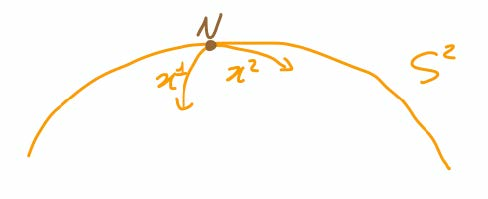
\includegraphics[width=4.5cm]{../img/north-angular-coordi.jpg}}\vspace{-0.4cm}
\]

In order to redefine the one form we can either using the Jacobian or notice that exterior derivative of $\tan\theta$ can be used to substitute $\de\phi$ with the new coordinates:
\[\de\tan\phi=(1+\tan^2\phi)\de\phi=\p{1+\p{\frac{x^2}{x^1}}^2}\de\phi=-\frac{x^2}{(x^1)^2}\de x^1+\frac1{x^1}\de x^2\]
hence we obtain
\[\psi_1=-\frac{\sqrt{1-(x^1)^2-(x^2)^2}}{(x^1)^2+(x^2)^2}(-x^2\de x^1+x^1\de x^2)\]
Now its clear that $\psi_1$ is singular for $(x^1,x^2)=(0,0)$. 

Let's consider now the 2-form 
\[\omega_2=\frac12\widetilde\omega_{\mu\nu}\de\tilde x^\mu\wedge\de \tilde x^\nu=\sin\theta\,\de\theta\wedge\de\phi\]
We can easily prove that it is smooth on the poles. Notice that $\de\omega_2=0$ (is a 3-form in a 2-dim manifold) hence $\omega_2$ is closed. By Poincaré lemma it is also locally exact, indeed in $S^2\setminus\{\text{poles}\}$ we have
\[\de\psi_1=\de(-\cos\,\theta\de\phi)=\sin\theta\,\de\theta\wedge\de\phi=\omega_2\]
But $\psi_1$ is not defined at poles, indeed $\omega_2$ is only locally exact. 

\end{example}



\section{Manifolds with metric}

Manifolds do not carry natural notions of 
\begin{enumerate}[ label=\textbullet]
\item length and volumes
\item notions of spatial and temporal ``directions''
\item a way to distinguish the locally inertial/freely falling frames
\end{enumerate}
All this notion are given by the introduction of a metric:

\begin{definition}[Metric]{}

The \textbf{metric} is a tensor field
\[g(x)=g_{\mu\nu}(x)\de x^\mu\otimes\de x^\nu\]
which satisfy following proprieties: it is symmetric
\[g_{\mu\nu}(x)=g_{\nu\mu}(x)=g_{(\mu\nu)}(x)\]
and it is non-degenerate
\[\det(g_{\mu\nu})\neq0\]
Its content is equivalently encoded in the \textbf{line element}, since thanks to symmetry we can omit tensorial product symbol
\[\boxed{\de s^2=g_{\mu\nu}(x)\de x^\mu\de x^\nu}\]
therefore usually we use terms ``metric'' and ``line element'' with the same meaning. 

The metric takes values in $T*M\otimes_ST*M$ and can be regarded as defining a scalar product
\[g(V,W)=g_{\mu\nu}(x)V^\mu(x)W^\nu(x)\]
which associate to two vector fields a scalar field. This also implies that the scalar product is invariant. We can also define the ``lenght'' of a vector, i.e. introduce a \textbf{norm}, given by $g(V,V)$. Generalizing what we stated for SR we say
\begin{enumerate}
\item if $G(V,V)>0$ then $V^\mu$ is \textbf{space-like}
\item if $G(V,V)<0$ then $V^\mu$ is \textbf{time-like}
\item if $G(V,V)=0$ then $V^\mu$ is \textbf{null} (or \textbf{light-like})
\end{enumerate}
An \textbf{Euclidean / Riemannian (metric) space} $\mathcal M_d$ is a manifold equipped to a metric such then all vectors are space-like, i.e. $g$ is positive definite everywhere. A\textbf{Lorenzian / Minkowskian / pseudo-Riemannian (metric) space(-time)} $\mathcal M_d$  is a manifold equipped to a metric $g$ which has $d-1$ positive eigenvalues and 1 negative eigenvalues (strictly, there are no zero eigenvalues). Negative eigenvalues corresponds to time direction, while positive eigenvalues corresponds to spatial directions. Can be proved that the characterization of the metric in terms of signature of its eigenvalues (this is called the \textbf{signature} of the metric) is invariant under change of coordinates, i.e. do not depends by the parametrization of the manifold. 

\end{definition}

Regarding $g_{\mu\nu}$ as a symmetric matrix, we can find an orthogonal matrix $E$ ($E^TE=\id$) such that
\[E^TgE=\text{diag}(\lambda_0,\dots,\lambda_{d+1})\]
with $\lambda_i\neq0$. Then previous condition implies
\[g_{\mu\nu}{E^\mu}_a{E^\nu}_b=\lambda_a\delta_{ab}\]
where in the last term there is no summation over index $a$. Once we identified the matrix $E$ we can define basis
\[{e^\mu}_a=\frac1{\sqrt{|\lambda_a|}}{E^\mu}_a\]
so that 
\[e^Tge=g_{\mu\nu}{e^\mu}_a{e^\mu}_b=\text{diag}(-1,\dots,-1,1,\dots,1)\]
and in particular for the Lorenzian spacetime we have $e^Tge=\text{diag}(-1,1,\dots,1)$.
Hence \textit{a metric space(-time) is Lorenzian iff exists an orthonormal basis $e_a=e_a^\mu\partial_\mu$ such that }
\[\boxed{g_{\mu\nu}{e^\mu}_a{e^\nu}_b=\eta_{ab}$ \qquad\text{with}\quad $\eta_{ab}=\text{diag}(-1,1,\dots,1)}\]
By introducing a dual basis of 1-forms $e^a={e^a}_\mu\de x^\mu$ such that $e^a_\mu e^\mu_b=\delta^a_b\Leftrightarrow e^a_\mu e^\nu_a=\delta_\mu^nu$ then we can equivalently say that \textit{the metric space(-time) is Lorenzian iff exists an orthonormal basis $e^a=e^a_\mu\de x^\mu$ such that}
\[\boxed{
g_{\mu\nu}=\eta_{ab}e^a_\mu e^b_\nu\quad\Leftrightarrow\quad g=\eta_{ab}e^a\otimes e^b\quad\Leftrightarrow\quad \de s^2=\eta_{ab}e^a e^b}\]
Basis $e_a$ and $e^a$ are often called \textbf{Lorentz / flat (co)frames} but notice that they exists only point-wise and, generically, they do not correspond to inertial coordinate systems $\hat x^\alpha$ such that 
\begin{equation}\label{eqn:coord-inert-frame}
e^a=\delta^a_\alpha\de\hat x^\alpha\quad\Leftrightarrow\quad \hat e^a_\alpha(\hat x)=\delta_\alpha^a\quad\Leftrightarrow\quad \de s^2=\eta_{\alpha\beta}\de\hat x^\alpha\de\hat x^\beta
\end{equation}
On the other hand we will see that for generic ``curved'' space-times condition eq.~\eqref{eqn:coord-inert-frame} can be satisfied only ``locally'' through a proper choice of coordinates
\[\boxed{
\de s^2=\left[\eta_{\alpha\beta}+O\p{\frac{\Delta\hat x^2}{L^2}}\right]\de\hat x^\alpha\de\hat x^\beta
}\]
where the second order term cannot vanishes since it contains the information about the curvature.\footnote{See \textsf{Carrol} pag. 74 for an explanation about why this is the better result one can archive.} Coordinates which satisfies this condition are called \textbf{``local'' inertial coordinates}.



\begin{example}[(Euclidean) round metric on $S^n$]
If we consider $S^n$ embedded into $\mathbb E^{n+1}$ 
\begin{figure}[H]
\centering
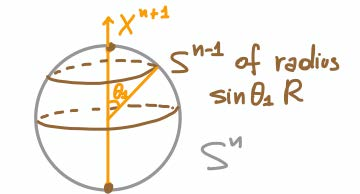
\includegraphics[width=4cm]{../img/round-metric-sn.jpg}
\end{figure}
then the round metric is inherited from the ambient flat metric
\[\de s^2(\mathbb E^{n+1})=(\de x^1)^2+\dots+(\de x^{n+1})^2\]
We can introduce angular coordinates by iteration, starting from $\theta_1$ we have
\[\de s^2(S^n)=R^2[\de\theta_1^2+\sin^2\theta_1\de s^2(S^{n-1})]\]

In order to prove this (left as an exercize) it is easier to start with the explicit computation of $\de s^2(S^2)$ and $\de s^2(S^3)$. 

\end{example}


In any metric space one can use the metric $g_{\mu\nu}$ or its inverse $g^{\mu\nu}$ to lower or raise the indices of any tensor, for instance
\[{T^\mu}_\nu\quad\longrightarrow\quad T_{\mu\nu}\equiv g_{\mu\rho}{T^\rho}_\nu\]
In the following we will consider this identifications as implicit. However one should keep in mind that, being $G_{\mu\nu}(x)$ an elementary dynamical field in GR, ${T^\mu}_\nu(x)$ and $T_{\mu\nu}(x)$ may carry different physical content.

\subsubsection{Interpretation of one forms and line elements}
Let's give an interpretation of $\de x^\mu$. Consider an infinitesimal displacement 
\[x^\mu\quad\longrightarrow\quad x^\mu+\delta x^\mu\]
We could set $\delta x^\mu=\epsilon V^\mu$ with $V^\mu$ finite vector applied at $x^\mu$, then we can identify an infinitesimal vector as
\[\epsilon V=\epsilon V^\mu\partial_\mu=\delta x^\mu\partial_\mu\]
Hence, when we apply the one form $\de x^\mu$ to such infinitesimal vector, we have
\[\de x^\mu(\epsilon V)=\epsilon V^\mu\equiv\delta x^\mu\]
Provided some infinitesimal vector $\epsilon V$, this suggest following identification
\[\de x^\mu\quad\sim\quad\delta x^\mu\]
where $\de x^\mu$ can be interpret as generic variation of the coordinate along a vector $V$.

When we generalize this analysis to one forms associated to scalar fields we have
\[\de f(\epsilon V)=\partial_\mu f\de x^\mu(\epsilon V)=\epsilon V^\mu\partial_\mu f=\delta x^\mu\partial_\mu f=\delta f\]
then $\de f(\epsilon V)$ coincides to the infinitesimal variation of the scalar field $f$ corresponding to $\delta x^\mu$. Again, provided some infinitesimal vector, we have the following identification
\[\de f=\partial_\mu f\de x^\mu\quad\sim\quad\delta f=\partial_\mu f\delta x^\mu\]
where $\de f$ is the generic variation of $f$ while $\delta f$ is the specific variation of $f$ under $\delta x^\mu$.
 
 Let's see how this works for the metric. Given $\delta x^\mu=\epsilon V^\mu$, its infinitesimal interval is given by 
\[\delta s^2=g(\epsilon V,\epsilon V)=\epsilon ^2g_{\mu\nu}V^\mu V^\nu=g_{\mu\nu}\delta x^\mu\delta x^\nu\]
And, provided an infinitesimal vector, we have the identification
\[\de s^2=g_{\mu\nu}\de x^\mu\de x^\nu\quad\sim\quad\delta s^2=g_{\mu\nu}\delta x^\mu\delta x^\nu\]
where $\de s^2$ is a generic infinitesimal interval, wile $\delta s^2$ is the specific interval of $\delta x^\mu=\epsilon V^\mu$.\\

\begin{example}[The evolving universe]

\textsf{Carroll, sec 2.6, 8.2, 8.4}\\

Let's consider a family of metrics that plays a special role in the description of expanding universe:
\begin{equation}\label{eqn:metric-exp-univ}
\de s^2=-\de t^2+a^2(t)\de\vec x\cdot\de\vec x=-\de t^2+a^2(t)\delta_{ij}\de x^i\de x^j
\end{equation}
Metrics in this forms are a subclass of the \emph{Friedmann-Robertson-Walker (FRW) space-times}.
Notice that  $t$ is the proper time measured by clock stuck at constant position $\vec x$, this is a consequence of the fact that the only term related to the time in the line element is $-\de t^2$ as in the flat metric.  

On the other hand, the proper distance between simultaneous events scale as $a(t)$, which cannot be absorbed by change coordinates since it is a time dependent factor.  
The distance between two events in world line of observers placed in fixed positions $x_a$ and $x_B$ is 
\[\Delta L=a(t)\vert\vec x_B-\vec x_A\vert
\hspace{1cm}
\raisebox{-2.4cm}{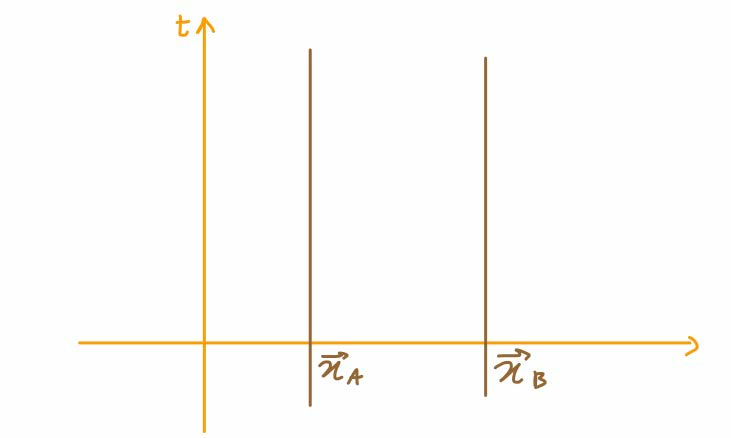
\includegraphics[width=5.5cm]{../img/world-lines-expand-univ.jpg}}\]
For this reason the factor $a(t)$ is called \textbf{scale factor}. In GR factor $a(t)$ is fixed by Einstein equations, and describes the expansion of universe. 
Anyhow just assuming homogeneous and isotropic distribution of matter and radiation one obtain a power law relation for $a(t)$:
\[a(t)=\p{\frac t{t_*}}^q\qquad0\leq q<1\quad
\begin{cases}
q=\frac23\quad\text{matter dominated universe}\\
q=\frac12\quad\text{rafiation dominated universe}
\end{cases}\]
where $t_*$ is a typical time scale characterizing the phase of cosmological evolution.
With such a a power low dependence, for $t\to 0$ we have $a(t)\to0$, hence metric looks singular and this singularity does not depend on the choice of parametrization, it is intrinsic in the geometry of the manifold. For this reason is a \emph{proper} singularity called \emph{Big Bang}.

Nowadays this idea has been overcome, in particular in the early period of cosmological evolution is characterized by a \textbf{period of inflation}, and in such period one can approximate scale factor as
\begin{equation}\label{eqn:Hubble-acceler}
\boxed{a(t)=e^{Ht}}
\end{equation}
where $t_*$ is called \textbf{Hubble scale} and $H=1/t*$ is the \textbf{Hubble parameter}. In this way the Big Bang singularity is pushed to $t=-\infty$.

The cosmological solution with $A(t)=e^{Ht}$ describes a patch of the 4-dimensional de Sitter space $\text{dS}_4\subset\mathbb M_5$ with equation
\begin{equation}\label{eqn:de-Sitter-eqn}
\vert\vec X\vert^2-T^2=L^2
\end{equation}
where $\vec X=(X^1,\dots,X^4)$.
\begin{figure}[H]
\centering
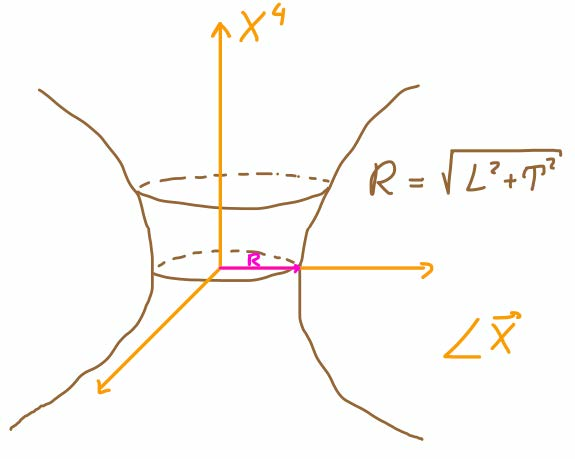
\includegraphics[width=5cm]{../img/de-Sitter-expanding-univ.jpg}
\end{figure}
\noindent
The flat metric $\mathbb M_5$ induces a metric on $\text{dS}_4$
\[\text{dS}_4(\textbb{M_5})-\de T^2+\de \vec X\cdot \de\vec X\]
In order to solve eq.~\eqref{eqn:de-Sitter-eqn} one may set
\begin{align*}
T&=L\sinh\p{\frac tL}+\frac12\frac{|\vec x|^2}Le^{t/L}\\
X^4&=L\cosh\p{\frac tL}-\frac12\frac{|\vec x|^2}Le^{t/L}\\
X^i&=x^ie^{t/L}\qquad i=1,2,3
\end{align*}
where $\vec x=(x^1,x^2,x^3)$, then one obtain\footnote{Prove it as exercise} that the line element induced in the de Sitter space is eq.~\eqref{eqn:metric-exp-univ} with eq.~\eqref{eqn:Hubble-acceler} and $H=\frac12$. 

Moreover, the patch covered by cosmological coordinates does not cover the full de Sitter space, but only half of it
\begin{figure}[H]
\centering
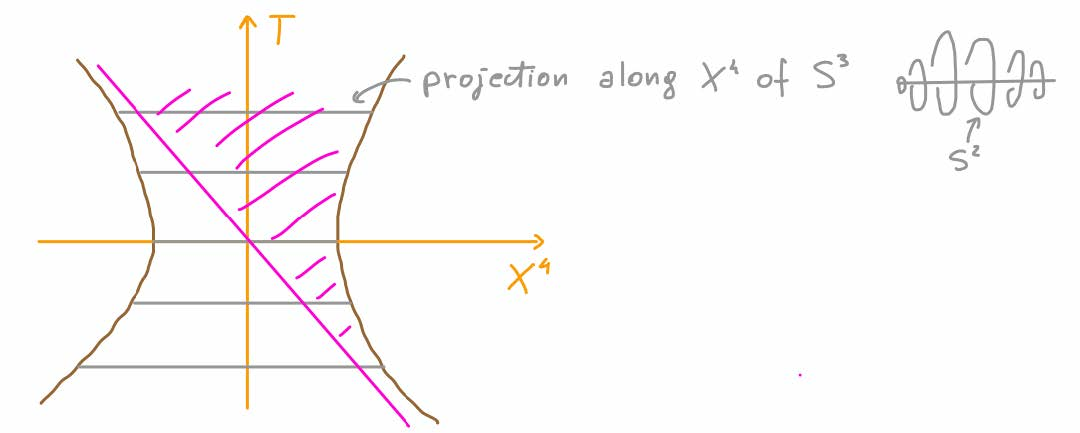
\includegraphics[width=10cm]{../img/patch-de-Sitter-expand-univ.jpg}
\end{figure}


\end{example}

\end{document}